\chapter{RESULTS}
\section{Tabular Results} 
We have set the maximum amount of generations to 24, as we have observed 
that the AI often does not evolve any further after the 24th generation. The 
table \ref{table:CPU vs GPU total runtime} and 
\ref{table:CPU vs GPU total runtime part 2} contains the total time in each
run per seed for both CPU and GPU. The ANOVA test indicates that the result
we got was not a type 1 error as shown in figure \ref{fig:anova_result}.
\begin{figure}
	\centering
		\graphicspath{{images/}}
		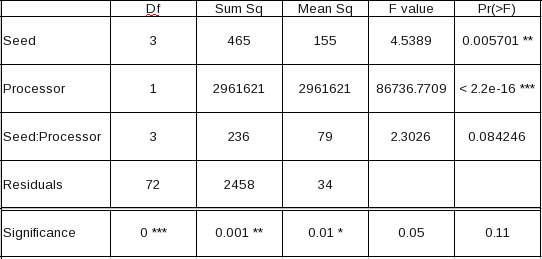
\includegraphics[width=260 pt]{Anova_Results.png}
	\caption{Anova Results}
	\label{fig:anova_result}
\end{figure}
Thus, the GPU can be considered to be faster than the CPU as shown in figure
\ref{fig:anova_result_graph}.
\begin{figure}
	\centering
		\graphicspath{{images/}}
		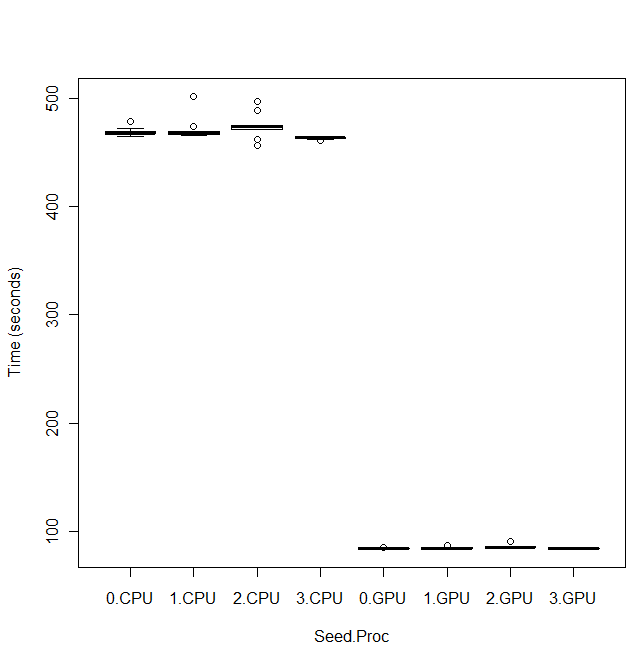
\includegraphics[width=260 pt]{Anova_Result_Graph.png}
	\caption{CPU vs GPU Graph}
	\label{fig:anova_result_graph}
\end{figure}

\begin{table}
\caption{CPU vs GPU Total Runtime Seeds 0 and 1}
\centering
 \begin{longtable}{ | l | l | l |}
    \hline
    Time & Seed & Processor \\ \hline
    471.94 & 0 & CPU \\ \hline
    469.5 & 0 & CPU \\ \hline
    468.12 & 0 & CPU \\ \hline
    468 & 0 & CPU \\ \hline
    478.42 & 0 & CPU \\ \hline
    467.59 & 0 & CPU \\ \hline
    465.22 & 0 & CPU \\ \hline
    465.5 & 0 & CPU \\ \hline
    467.64 & 0 & CPU \\ \hline
    467.19 & 0 & CPU \\ \hline
    85 & 0 & GPU \\ \hline
    83.96 & 0 & GPU \\ \hline
    84.07 & 0 & GPU \\ \hline
    83.91 & 0 & GPU \\ \hline
    83.99 & 0 & GPU \\ \hline
    83.94 & 0 & GPU \\ \hline
    83.95 & 0 & GPU \\ \hline
    83.96 & 0 & GPU \\ \hline
    83.93 & 0 & GPU \\ \hline
    83.93 & 0 & GPU \\ \hline
    469.11 & 1 & CPU \\ \hline
    466.16 & 1 & CPU \\ \hline
    466.18 & 1 & CPU \\ \hline
    468.07 & 1 & CPU \\ \hline
    465.86 & 1 & CPU \\ \hline
    466.64 & 1 & CPU \\ \hline
    467.87 & 1 & CPU \\ \hline
    468.76 & 1 & CPU \\ \hline
    473.68 & 1 & CPU \\ \hline
    501.45 & 1 & CPU \\ \hline
    83.97 & 1 & GPU \\ \hline
    84.79 & 1 & GPU \\ \hline
    83.78 & 1 & GPU \\ \hline
    83.83 & 1 & GPU \\ \hline
    83.87 & 1 & GPU \\ \hline
    83.85 & 1 & GPU \\ \hline
    83.88 & 1 & GPU \\ \hline
    83.8 & 1 & GPU \\ \hline
    86.9 & 1 & GPU \\ \hline
    86.91 & 1 & GPU \\ \hline
    \end{longtable}
\label{table:CPU vs GPU total runtime}
\end{table}
\bigskip

\begin{table}
\caption{CPU vs GPU Total Runtime Seeds 2 and 3}
\centering
 \begin{longtable}{ | l | l | l |}
    \hline
    Time & Seed & Processor \\ \hline
    497.14 & 2 & CPU \\ \hline
    462.1 & 2 & CPU \\ \hline
    456.83 & 2 & CPU \\ \hline
    489.04 & 2 & CPU \\ \hline
    472.8 & 2 & CPU \\ \hline
    471.66 & 2 & CPU \\ \hline
    473.58 & 2 & CPU \\ \hline
    474.54 & 2 & CPU \\ \hline
    474.99 & 2 & CPU \\ \hline
    474.22 & 2 & CPU \\ \hline
    86.13 & 2 & GPU \\ \hline
    90.46 & 2 & GPU \\ \hline
    90.48 & 2 & GPU \\ \hline
    85.75 & 2 & GPU \\ \hline
    84.77 & 2 & GPU \\ \hline
    84.96 & 2 & GPU \\ \hline
    85.06 & 2 & GPU \\ \hline
    84.92 & 2 & GPU \\ \hline
    84.96 & 2 & GPU \\ \hline
    86.18 & 2 & GPU \\ \hline
    461.94 & 3 & CPU \\ \hline
    464.13 & 3 & CPU \\ \hline
    464.6 & 3 & CPU \\ \hline
    461.13 & 3 & CPU \\ \hline
    464.12 & 3 & CPU \\ \hline
    463.9 & 3 & CPU \\ \hline
    463.06 & 3 & CPU \\ \hline
    464.25 & 3 & CPU \\ \hline
    463.54 & 3 & CPU \\ \hline
    464.36 & 3 & CPU \\ \hline
    84.22 & 3 & GPU \\ \hline
    84.27 & 3 & GPU \\ \hline
    84.24 & 3 & GPU \\ \hline
    84.24 & 3 & GPU \\ \hline
    84.27 & 3 & GPU \\ \hline
    84.25 & 3 & GPU \\ \hline
    84.2 & 3 & GPU \\ \hline
    84.23 & 3 & GPU \\ \hline
    84.28 & 3 & GPU \\ \hline
    84.22 & 3 & GPU \\ \hline
    \end{longtable}
\label{table:CPU vs GPU total runtime part 2}
\end{table}
\bigskip


